% ============================================================
%  Chapter 1: Introduction + Mappings & Functions
%  Source: Tongji 8th-edition courseware (black-white)
%  D1_0 Introduction + D1_1 Mappings and Functions
%  English Beamer lecture slides — step-by-step examples via \pause
% ============================================================
\documentclass[aspectratio=169,10pt]{beamer}

\usetheme{Madrid}
\usecolortheme{default}
\usepackage{amsmath,amssymb,amsthm}
\usepackage{mathtools}
\usepackage{tikz}
\usetikzlibrary{shapes,arrows.meta,positioning,calc}

\title{Chapter 1: Analytical Foundations}
\subtitle{Introduction \& Mappings and Functions}
\author{Advanced Mathematics \\ (Tongji University, 8th Ed.)}
\date{}
\institute{}

% ------------------------------------------------------------
\begin{document}

% ==================== TITLE ====================
\begin{frame}
  \titlepage
\end{frame}

% ==================== TABLE OF CONTENTS ====================
\begin{frame}{Outline}
  \tableofcontents
\end{frame}

% ############################################################
\section{Introduction to the Course}
% ############################################################

% -------------------- Textbook & References --------------------
\begin{frame}{Textbook \& References}
  \begin{block}{Main Textbook}
    \textit{Advanced Mathematics} (8th Edition)\\
    Department of Applied Mathematics, Tongji University\\
    Higher Education Press, 2020.
  \end{block}
  \pause
  \begin{block}{Supplementary Reading}
    \textit{Solutions Manual for Advanced Mathematics (8th Ed., Combined Volume)}\\
    China Water \& Power Press, 2021.
  \end{block}
\end{frame}

% -------------------- Course Content Overview --------------------
\begin{frame}{Course Content Overview}
  \begin{enumerate}
    \item<1-> \textbf{Analytical Foundations:} Functions, Limits, Continuity
    \item<2-> \textbf{Calculus of One Variable} (Volumes I \& II)
    \item<3-> \textbf{Vector Algebra \& Analytic Geometry in Space}
    \item<4-> \textbf{Infinite Series}
    \item<5-> \textbf{Ordinary Differential Equations}
  \end{enumerate}
  \vfill
  \onslide<6->{\centering\small
    Multivariable Calculus is covered in Volumes III--V.
  }
\end{frame}

% -------------------- How to Study --------------------
\begin{frame}{How to Study Advanced Math?}
  \begin{enumerate}
    \item<1-> Recognize the importance; cultivate strong interest.
    \pause
    \item<2-> The best way to learn mathematics is to \textbf{do} mathematics.
          \begin{quote}
            ``Genius lies in hard work; talent accumulates through study.''\\
            \hfill --- Hua Luogeng
          \end{quote}
    \pause
    \item<3-> Apply what you learn; create from what you master.\\
          Go from thin to thick, then from thick to thin.
  \end{enumerate}
  \vspace{4pt}
  \onslide<4->{
    \begin{alertblock}{Marx \& Engels on Mathematics}
      \scriptsize
      ``To understand nature dialectically\\
      and materially, one must be\\
      familiar with mathematics.''\\ --- Engels\\[2pt]
      ``A science reaches true perfection\\
      only when it employs\\
      mathematics.''\\ --- Marx
    \end{alertblock}
  }
\end{frame}

% ############################################################
\section{Mappings and Functions}
% ############################################################

% -------------------- Section Title --------------------
\begin{frame}
  \centering
  \vfill
  {\Large\bfseries Section 1: Mappings and Functions}\\[8pt]
  {\large I.\ Mappings \quad\quad II.\ Functions}
  \vfill
\end{frame}

% -------------------- Intro Examples --------------------
\begin{frame}{Motivating Examples for Mappings}
  \begin{example}[Addition of $x$ and $\sin x$]
    For every $x\in\mathbb{R}$,
    \[
      y = x + \sin x
    \]
    defines a mapping from $\mathbb{R}$ to $\mathbb{R}$.
  \end{example}
  \pause
  \begin{center}
    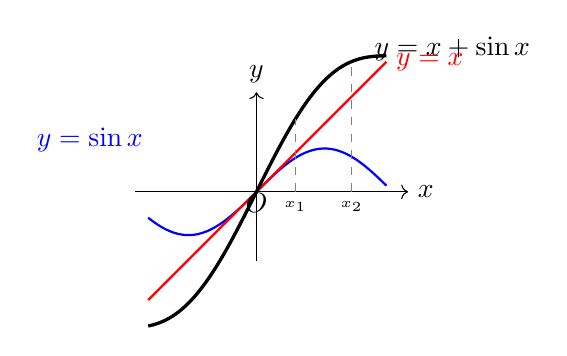
\begin{tikzpicture}[scale=0.55]
      \draw[->] (-2.8,0) -- (3.5,0) node[right] {$x$};
      \draw[->] (0,-1.6) -- (0,2.3) node[above] {$y$};
      % y = sin x (blue)
      \draw[thick,blue,domain=-2.5:3,samples=80] plot (\x,{sin(\x r)});
      % y = x (red)
      \draw[thick,red] (-2.5,-2.5) -- (3,3);
      % y = x + sin x (black thick)
      \draw[very thick,black,domain=-2.5:3,samples=80] plot (\x,{\x+sin(\x r)});
      \node[red,right] at (3,3) {$y=x$};
      \node[blue,left] at (-2.4,1.2) {$y=\sin x$};
      \node[black,above right] at (2.5,2.8) {$y=x+\sin x$};
      \node at (0,-0.25) {$O$};
      % vertical markers at x1, x2
      \draw[dashed,gray] (0.9,0)--(0.9,{0.9+sin(0.9 r)});
      \draw[dashed,gray] (2.2,0)--(2.2,{2.2+sin(2.2 r)});
      \node[below,font=\tiny] at (0.9,0) {$x_1$};
      \node[below,font=\tiny] at (2.2,0) {$x_2$};
    \end{tikzpicture}
  \end{center}
\end{frame}

% -------------------- Circle Projection Example --------------------
\begin{frame}{Example: Projection onto the $y$-axis}
  Let
  \[
    C = \{(x,y)\mid x^2+y^2=1\}\quad\text{(unit circle)},\qquad
    Y = \{(0,y)\mid -1\le y\le 1\}.
  \]
  \pause
  For every point $P\in C$, project orthogonally onto the $y$-axis
  to obtain $Q\in Y$. This defines a mapping $C\to Y$.
  \pause
  \begin{columns}
    \column{0.45\textwidth}
    \begin{center}
      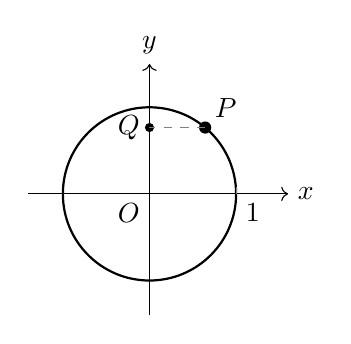
\begin{tikzpicture}[scale=1.1]
        \draw[->] (-1.4,0) -- (1.6,0) node[right] {$x$};
        \draw[->] (0,-1.4) -- (0,1.5) node[above] {$y$};
        \draw[thick] (0,0) circle (1);
        % Point P on circle
        \coordinate (P) at ({cos(50)},{sin(50)});
        \fill (P) circle (2pt) node[above right] {$P$};
        % Projection Q on y-axis
        \coordinate (Q) at (0,{sin(50)});
        \fill (Q) circle (1.5pt) node[left] {$Q$};
        % Dashed line
        \draw[dashed,gray] (P) -- (Q);
        % Labels
        \node[below left] at (0,0) {$O$};
        \node[below right] at (1,0) {$1$};
        \draw[dashed,gray] (1,0) -- (1,0.08);
      \end{tikzpicture}
    \end{center}
    \column{0.52\textwidth}
    \small
    \textbf{Properties:}
    \begin{itemize}
      \item This mapping is \alert{surjective}: every $Q\in Y$ has a pre-image.
      \item It is \alert{not injective}: two symmetric points $P$, $P'$ map to the same $Q$.
    \end{itemize}
  \end{columns}
\end{frame}

% -------------------- Definition of Mapping --------------------
\begin{frame}{Definition of a Mapping}
  \begin{definition}[Mapping]
    Let $X$ and $Y$ be two nonempty sets.
    If there exists a rule $f$ such that
    \[
      \forall\, x\in X,\;\exists\;\text{a unique } y\in Y \text{ corresponding to } x,
    \]
    then $f$ is called a \textbf{mapping} from $X$ to $Y$, denoted
    \[
      f\colon X \longrightarrow Y,\qquad y = f(x).
    \]
  \end{definition}
  \pause
  \begin{itemize}
    \item $y = f(x)$: the \textbf{image} of $x$ under $f$.
    \item $x$: a \textbf{pre-image} of $y$ under $f$ (not necessarily unique!).
    \item $X$: the \textbf{domain} of $f$.
    \item $R_f = f(X) = \{\,f(x)\mid x\in X\,\}$: the \textbf{range} of $f$.
  \end{itemize}
  \pause
  \begin{alertblock}{Three Elements of a Mapping}
    Domain, Correspondence Rule, Range.
  \end{alertblock}
\end{frame}

% -------------------- Surjection / Injection / Bijection --------------------
\begin{frame}{Types of Mappings}
  For a mapping $f\colon X\to Y$:
  \pause
  \begin{description}
    \item[Surjective (onto)] if $f(X) = Y$. \hfill {\small (every $y\in Y$ has a pre-image)}
    \pause
    \item[Injective (one-to-one)] if $\forall x_1,x_2\in X$, $x_1\neq x_2 \Rightarrow f(x_1)\neq f(x_2)$.
          \hfill {\small (distinct inputs give distinct outputs)}
    \pause
    \item[Bijective] if $f$ is both surjective and injective.
  \end{description}
  \pause
  \vspace{4pt}
  \begin{center}
    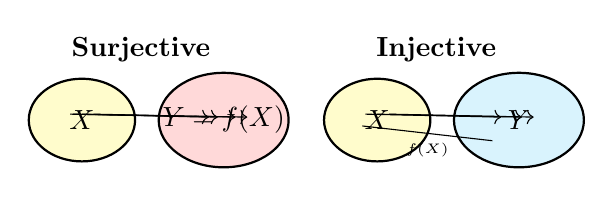
\begin{tikzpicture}[scale=0.75]
      % Surjection
      \node at (-3.2,1.2) {\textbf{Surjective}};
      \draw[thick,fill=yellow!20] (-4.2,0) ellipse (0.9 and 0.7);
      \node at (-4.2,0) {$X$};
      \draw[thick,fill=red!15] (-1.8,0) ellipse (1.1 and 0.8);
      \node at (-1.8,0) {$Y=f(X)$};
      \foreach \a/\b in {-4.4/-1.4, -4.2/-1.9, -4.0/-1.6, -4.35/-2.05}{
        \draw[->] (\a,0.1) -- (\b,0.05);
      }
      % Injection
      \node at (1.8,1.2) {\textbf{Injective}};
      \draw[thick,fill=yellow!20] (0.8,0) ellipse (0.9 and 0.7);
      \node at (0.8,0) {$X$};
      \draw[thick,fill=cyan!15] (3.2,0) ellipse (1.1 and 0.8);
      \node at (3.2,0) {$Y$};
      \foreach \a/\b in {0.6/2.9, 0.8/3.25, 1.0/3.45}{
        \draw[->] (\a,0.1) -- (\b,0.05);
      }
      \draw (0.55,-0.1) -- (2.75,-0.35) node[midway,below]{\tiny $f(X)$};
    \end{tikzpicture}
  \end{center}
\end{frame}

% -------------------- Examples of Mappings (1/2) --------------------
\begin{frame}{Examples of Mappings \textnormal{(I)}}
  \begin{example}[Heron's Formula --- Surjective]
    For every triangle $\Delta$ in the set of all triangles,
    \[
      S = \sqrt{p(p-a)(p-b)(p-c)},\quad p=\tfrac12(a+b+c)
    \]
    maps $\Delta$ to its area $S\in(0,+\infty)$.
    This mapping is \textbf{surjective}.
  \end{example}
  \pause
  \begin{columns}
    \column{0.42\textwidth}
    \begin{center}
      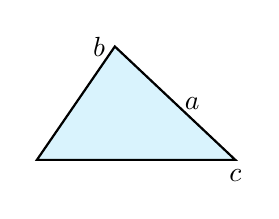
\begin{tikzpicture}[scale=0.9]
        % Triangle
        \coordinate (A) at (0,0);
        \coordinate (B) at (2.8,0);
        \coordinate (C) at (1.1,1.6);
        \draw[thick,fill=cyan!15] (A)--(B)--(C)--cycle;
        \node[below] at (A) {};
        \node[below] at (B) {$c$};
        \node[left]  at (C) {$b$};
        \node[right] at (1.95,0.8) {$a$};
      \end{tikzpicture}
    \end{center}
    \column{0.55\textwidth}
    \begin{example}[Area Under $e^x$ --- Surjective]
      For each $x\in[0,+\infty)$:
      \[
        S(x)=\int_0^x e^t\,dt = e^x-1.
      \]
      $S\in[0,+\infty)$ is surjective onto itself.
    \end{example}
  \end{columns}
\end{frame}

% -------------------- Examples of Mappings (2/2) --------------------
\begin{frame}{Examples of Mappings \textnormal{(II)}}
  \begin{example}[Polar-to-Cartesian --- Surjective]
    \[
      f\colon [0,+\infty)\times[0,2\pi) \longrightarrow \mathbb{R}^2,\quad
      \begin{cases}
        x = r\cos\theta,\\
        y = r\sin\theta,
      \end{cases}
    \]
    is surjective (covers the whole plane).
  \end{example}
  \pause
  \begin{center}
    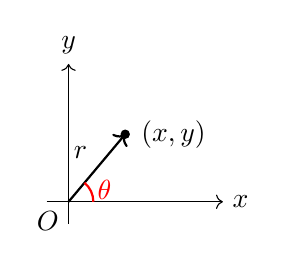
\begin{tikzpicture}[scale=0.7]
      \draw[->] (-0.4,0) -- (2.8,0) node[right] {$x$};
      \draw[->] (0,-0.4) -- (0,2.5) node[above] {$y$};
      % Ray from origin
      \draw[thick,->] (0,0) -- ({1.6*cos(50)},{1.6*sin(50)}) node[circle,fill,inner sep=1.2pt,label=right:{$(x,y)$}]{};
      % Angle arc
      \draw[thick,red] (0.45,0) arc (0:50:0.45);
      \node[red] at (0.65,0.22) {$\theta$};
      % Radius label
      \node[above left] at ({0.8*cos(50)},{0.8*sin(50)}) {$r$};
      \node[below left] at (0,0) {$O$};
    \end{tikzpicture}
  \end{center}
\end{frame}

% -------------------- Special Names --------------------
\begin{frame}{Special Names for Mappings}
  Depending on the nature of $X$ and $Y$:
  \pause
  \begin{center}
    \renewcommand{\arraystretch}{1.4}
    \begin{tabular}{ccl}
      $X$ (set) & $Y$ (set) & Name of $f$ \\
      \hline
      any nonempty $\neq\varnothing$ & number set & \textbf{functional} \\
      any nonempty $\neq\varnothing$ & $X$ itself & \textbf{transformation / operator} \\
      number subset $D\subset\mathbb{R}$ & $\mathbb{R}$ & \textbf{function} \\
    \end{tabular}
  \end{center}
  \pause
  \vspace{6pt}
  \begin{block}{Key Point}
    A \textbf{function} is precisely a mapping whose domain is a subset of $\mathbb{R}$ and whose codomain is $\mathbb{R}$.
  \end{block}
\end{frame}

% -------------------- Inverse Mapping --------------------
\begin{frame}{Inverse Mapping}
  \begin{definition}[Inverse Mapping]
    Let $f\colon X\to Y$ be \textbf{injective}. Then for each $y\in R_f$
    there exists a unique $x\in X$ with $f(x)=y$.
    \pause
    We define a new mapping $g\colon R_f\to X$ by $g(y)=x$ where $f(x)=y$.
    This $g$ is called the \textbf{inverse mapping} of $f$, denoted $f^{-1}$:
    \[
      D_{f^{-1}} = R_f,\qquad R_{f^{-1}} = X.
    \]
  \end{definition}
  \pause
  \begin{alertblock}{Important}
    Only \textbf{injective} mappings admit an inverse!
  \end{alertblock}
\end{frame}

% -------------------- Example: Inverse Sine --------------------
\begin{frame}{Example: Principal Value of Arcsine}
  \begin{example}
    Let $f(x)=\sin x,\; x\in\bigl[-\frac{\pi}{2},\frac{\pi}{2}\bigr]$.
    \pause
    The inverse function is
    \[
      f^{-1}(x) = \arcsin x,\quad x\in[-1,1],
    \]
    called the \textbf{principal value of arcsine}.
    \pause
    \begin{itemize}
      \item Domain: $D_{f^{-1}}=[-1,1]$
      \item Range: $R_{f^{-1}}=\bigl[-\frac{\pi}{2},\frac{\pi}{2}\bigr]$
    \end{itemize}
  \end{example}
\end{frame}

% -------------------- Composite Mapping --------------------
\begin{frame}{Composite Mapping}
  \begin{definition}[Composite Mapping]
    Given two mappings $g\colon X\to Y_1$ and $f\colon Y_2\to Z$ with $Y_1\subseteq Y_2$,
    we define a mapping from $X$ to $Z$ by sending each $x\in X$ to $f[g(x)]\in Z$.
    \pause
    This is called the \textbf{composite} of $g$ and $f$, denoted $f\circ g$:
    \[
      (f\circ g)(x) = f(g(x)),\quad x\in X.
    \]
  \end{definition}
  \pause
  \begin{alertblock}{Condition for Composition}
    The range of $g$ must be contained in the domain of $f$:
    \[
      R_g \subseteq D_f.
    \]
  \end{alertblock}
\end{frame}

% -------------------- Composite Example --------------------
\begin{frame}{Example: Composition Order Matters}
  \begin{example}
    Let $f(x)=x^2$ and $g(x)=2x+1$.
    \pause
    \begin{itemize}
      \item $(f\circ g)(x) = f(g(x)) = (2x+1)^2 = 4x^2+4x+1$
      \pause
      \item $(g\circ f)(x) = g(f(x)) = 2x^2+1$
    \end{itemize}
    \pause
    Clearly $(f\circ g)(x) \neq (g\circ f)(x)$ in general.
  \end{example}
  \pause
  \begin{block}{Note}
    Composition is \textbf{not commutative}: order matters!
  \end{block}
\end{frame}

% ============================================================
\subsection{Functions}
% ============================================================

% -------------------- Function Definition --------------------
\begin{frame}{Definition of a Function}
  \begin{definition}[Function]
    Let $D\subset\mathbb{R}$ be a nonempty set.
    The mapping $f\colon D\to\mathbb{R}$ is called a \textbf{function} defined on $D$, written
    \[
      y = f(x),\quad x\in D.
    \]
  \end{definition}
  \pause
  \begin{itemize}
    \item $x$: \textbf{independent variable}
    \item $y$: \textbf{dependent variable}
    \item $D$: \textbf{domain}
    \item $R_f = f(D) = \{\,y\mid y=f(x),\, x\in D\,\}$: \textbf{range}
  \end{itemize}
  \pause
  \begin{block}{Graph of a Function}
    $C = \{\,(x,y)\mid y=f(x),\, x\in D\,\}\subset D\times f(D)$
  \end{block}
\end{frame}

% -------------------- Representations --------------------
\begin{frame}{Ways to Represent a Function}
  \begin{enumerate}
    \item<1-> \textbf{Analytic expression} (formula)
    \item<2-> \textbf{Graphical representation}
    \item<3-> \textbf{Tabular representation}
  \end{enumerate}
  \vfill
  \onslide<4->{
    \begin{example}[Absolute Value Function]
      $y = |x| = \begin{cases} x, & x\ge 0, \\ -x, & x<0. \end{cases}$
      \quad Domain $(-\infty,+\infty)$, Range $[0,+\infty)$
    \end{example}
  }
  \vfill
  \onslide<5->{
    \small
    \textbf{Domain convention:} For functions without a practical context, the domain is taken as the largest set where the expression makes sense.
    For applied problems, the domain must be stated explicitly.
  }
\end{frame}

% -------------------- Example 3: Piecewise Function --------------------
\begin{frame}{Example 3: Piecewise Function}
  \begin{example}
    Given $f(x)=\begin{cases}2\sqrt{x}, & 0\le x\le 1,\\ 1+x, & x>1.\end{cases}$
    \pause
    Find the domain, range, $f(\frac12)$, and $f(\frac1t)$.
  \end{example}
  \pause
  \begin{block}{Solution}
    Domain $D=[0,+\infty)$, \quad Range $f(D)=[0,+\infty)$.
    \pause
    \[
      f(\tfrac12) = 2\sqrt{\tfrac12} = \sqrt{2}.
    \]
    \pause
    \[
      f(\tfrac1t) =
      \begin{cases}
        1+\dfrac{1}{t}, & 0<t<1,\\[8pt]
        \dfrac{2}{\sqrt{t}},   & t\ge 1.
      \end{cases}
    \]
  \end{block}
\end{frame}

\begin{frame}{Example 3: Graph of the Piecewise Function}
  \begin{center}
    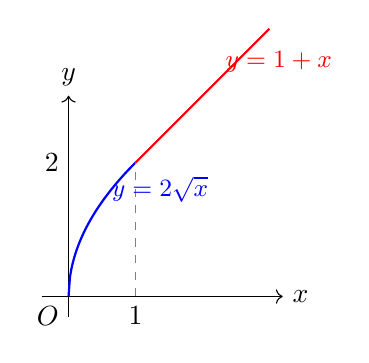
\begin{tikzpicture}[scale=0.85]
      \draw[->] (-0.4,0) -- (3.2,0) node[right] {$x$};
      \draw[->] (0,-0.3) -- (0,3) node[above] {$y$};
      % y = 2*sqrt(x) on [0,1]
      \draw[thick,blue,domain=0:1,samples=50] plot (\x,{2*sqrt(\x)});
      % y = 1+x on [1, 3]
      \draw[thick,red,domain=1:3,samples=30] plot (\x,{1+\x});
      % Dashed line at x=1
      \draw[dashed,gray] (1,0)--(1,2);
      \node[below] at (1,0) {$1$};
      \node[left] at (0,2) {$2$};
      % Labels
      \node[blue,right] at (0.5,1.6) {\small $y=2\sqrt{x}$};
      \node[red,right] at (2.2,3.5) {\small $y=1+x$};
      \node[below left] at (0,0) {$O$};
    \end{tikzpicture}
  \end{center}
\end{frame}

% ============================================================
\subsection{Properties of Functions}
% ============================================================

% -------------------- Boundedness --------------------
\begin{frame}{Boundedness}
  Let $y=f(x)$, $x\in D$, and $I\subset D$ be an interval.
  \pause
  \begin{definition}[Bounded]
    \begin{itemize}
      \item $f$ is \textbf{bounded on $D$} if $\exists\,M>0$ such that $|f(x)|\le M$ for all $x\in D$.
      \pause
      \item $f$ is \textbf{bounded on $I$} if $\exists\,M>0$ such that $|f(x)|\le M$ for all $x\in I$.
      \pause
      \item $f$ is \textbf{unbounded on $I$} if for every $M>0$ there exists $x\in I$ with $|f(x)|>M$.
    \end{itemize}
  \end{definition}
  \pause
  \begin{block}{Related Concepts}
    One can also define \emph{bounded above}, \emph{bounded below}, etc.\ (see p.~7).
  \end{block}
\end{frame}

% -------------------- Monotonicity --------------------
\begin{frame}{Monotonicity}
  For all $x_1,x_2\in I$ with $x_1<x_2$:
  \pause
  \begin{definition}[Monotone]
    \begin{itemize}
      \item If $f(x_1)<f(x_2)$, then $f$ is \textbf{strictly increasing} on $I$;
      \pause
      \item If $f(x_1)>f(x_2)$, then $f$ is \textbf{strictly decreasing} on $I$.
    \end{itemize}
  \end{definition}
  \pause
  \vspace{4pt}
  \begin{center}
    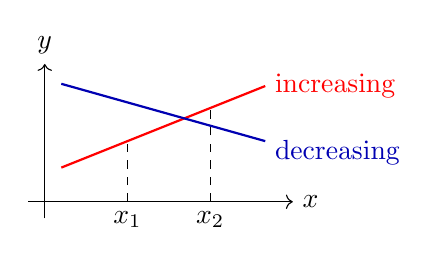
\begin{tikzpicture}[scale=0.7]
      \draw[->] (-0.3,0) -- (4.5,0) node[right] {$x$};
      \draw[->] (0,-0.3) -- (0,2.5) node[above] {$y$};
      \draw[thick,red] (0.3,0.62) -- (4,2.1);
      \draw[thick,blue!70!black] (0.3,2.14) -- (4,1.1);
      \draw[dashed] (1.5,0)--(1.5,1.1) (3,0)--(3,1.7);
      \node[below] at (1.5,0) {$x_1$}; \node[below] at (3,0) {$x_2$};
      \node[red,right] at (4,2.1) {increasing};
      \node[blue!70!black,right] at (4,0.9) {decreasing};
    \end{tikzpicture}
  \end{center}
\end{frame}

% -------------------- Even/Odd Parity --------------------
\begin{frame}{Even and Odd Functions}
  For all $x\in D$ such that $-x\in D$:
  \pause
  \begin{definition}[Parity]
    \begin{itemize}
      \item $f$ is \textbf{even} if $f(-x)=f(x)$;
      \pause
      \item $f$ is \textbf{odd} if $f(-x)=-f(x)$.
    \end{itemize}
  \end{definition}
  \pause
  \begin{alertblock}{Note}
    If an odd function is defined at $x=0$, then necessarily $f(0)=0$.
  \end{alertblock}
  \pause
  \begin{example}[Hyperbolic Cosine --- Even]
    \[
      y = \operatorname{ch}x = \frac{e^{x}+e^{-x}}{2},\qquad
      \operatorname{ch}(-x)=\operatorname{ch}x.
    \]
  \end{example}
\end{frame}

% -------------------- More Hyperbolic Examples --------------------
\begin{frame}{Hyperbolic Functions (cont.)}
  \begin{example}[Hyperbolic Sine --- Odd]
    \[
      y = \operatorname{sh}x = \frac{e^{x}-e^{-x}}{2},\qquad
      \operatorname{sh}(-x)=-\operatorname{sh}x.
    \]
  \end{example}
  \pause
  \begin{example}[Hyperbolic Tangent --- Odd]
    \[
      y = \operatorname{th}x = \frac{\operatorname{sh}x}{\operatorname{ch}x}
        = \frac{e^{x}-e^{-x}}{e^{x}+e^{-x}},\qquad
      \operatorname{th}(-x)=-\operatorname{th}x.
    \]
  \end{example}
  \pause
  \begin{block}{Even--Odd Decomposition}
    Any function $f$ defined on $(-l,l)$ can be decomposed as
    \[
      f(x) = \underbrace{\frac{f(x)+f(-x)}{2}}_{\text{even part}}
           + \underbrace{\frac{f(x)-f(-x)}{2}}_{\text{odd part}}.
    \]
  \end{block}
\end{frame}

% -------------------- Periodicity --------------------
\begin{frame}{Periodicity}
  \begin{definition}[Periodic Function]
    If $\forall\,x\in D$, $\exists\,l>0$ with $x\pm l\in D$ such that
    \[
      f(x\pm l) = f(x),
    \]
    then $f$ is called a \textbf{periodic function} and $l$ is a \textbf{period}\\
    (usually meaning the \emph{smallest positive period}).
  \end{definition}
  \pause
  \begin{columns}
    \column{0.48\textwidth}
    \begin{center}
      $y=|\sin x|$\\period $=\pi$\\[4pt]
      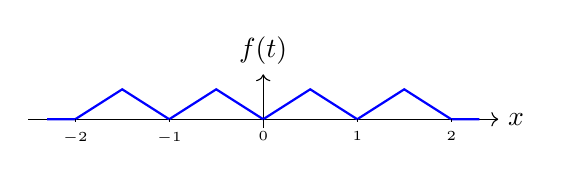
\begin{tikzpicture}[scale=0.38]
        \draw[->] (-2.5*pi,0) -- (2.5*pi,0) node[right]{$x$};
        \draw[->] (0,-0.3) -- (0,1.5) node[above]{$f(t)$};
        \draw[thick,blue] (-2.3*pi,0)--(-2*pi,0)--(-1.5*pi,1)--(-pi,0)--(-0.5*pi,1)--(0,0)
          --(0.5*pi,1)--(pi,0)--(1.5*pi,1)--(2*pi,0)--(2.3*pi,0);
        \foreach \s in {-2,-1,0,1,2}{\draw (\s*pi,0)--(\s*pi,-0.1) node[below]{\tiny$\s$};}
      \end{tikzpicture}
    \end{center}
    \column{0.48\textwidth}
    \begin{center}
      $y=\sin(\omega t)$\\period $=\dfrac{2\pi}{\omega}$\\[4pt]
      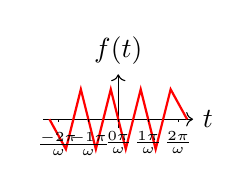
\begin{tikzpicture}[scale=0.38]
        \draw[->] (-2.5,0) -- (2.5,0) node[right]{$t$};
        \draw[->] (0,-0.3) -- (0,1.5) node[above]{$f(t)$};
        \draw[thick,red] (-2.3,0)--(-1.75,-1)--(-1.25,1)--(-0.75,-1)--(-0.25,1)
          --(0.25,-1)--(0.75,1)--(1.25,-1)--(1.75,1)--(2.3,0);
        \foreach \s in {-2,-1,0,1,2}{\draw (\s,0)--(\s,-0.1) node[below]{\tiny$\frac{\s\pi}{\omega}$};}
      \end{tikzpicture}
    \end{center}
  \end{columns}
\end{frame}

% -------------------- Periodicity: Counterexamples --------------------
\begin{frame}{Periodicity: Cautionary Notes}
  \begin{alertblock}{No Smallest Positive Period}
    Not every periodic function has a smallest positive period!
  \end{alertblock}
  \pause
  \begin{example}[Constant Function]
    $f(x)=C$ is periodic with \emph{every} positive number as a period.
  \end{example}
  \pause
  \begin{example}[Dirichlet Function]
    \[
      f(x) = \begin{cases}
        1, & x\text{ is rational},\\
        0, & x\text{ is irrational},
      \end{cases}
    \]
    is periodic with \emph{every rational} as a period --- no smallest positive period exists.
  \end{example}
\end{frame}

% ============================================================
\subsection{Inverse and Composite Functions}
% ============================================================

% -------------------- Inverse Function Concept --------------------
\begin{frame}{Inverse Functions}
  If $y=f(x)$ is injective on its domain, there exists an inverse mapping $f^{-1}$.
  \pause
  \begin{theorem}[Properties of Inverse Functions]
    \begin{enumerate}
      \item<2-> If $y=f(x)$ is strictly increasing (decreasing),\\
            then $f^{-1}(y)$ is also strictly increasing (decreasing).
      \item<3-> The graphs of $y=f(x)$ and $y=f^{-1}(x)$ are symmetric about the line $y=x$.
    \end{enumerate}
  \end{theorem}
  \pause\pause
  \begin{example}
    $y=e^x$ (exponential) and $y=\ln x$ (logarithm) are inverses of each other.\\
    Both are strictly increasing; their graphs are symmetric about $y=x$.
  \end{example}
\end{frame}

% -------------------- Composite Functions --------------------
\begin{frame}{Composite Functions}
  Given a function chain
  \[
    x \trightarrow{\;\text{\textcircled{1}}\;} u \trightarrow{\;\text{\textcircled{2}}\;} y,
  \]
  the composition yields $y=f[g(x)]$, where $u$ is the \textbf{intermediate variable}.
  \pause
  \begin{alertblock}{Composition Condition}
    The range of the inner function must lie within the domain of the outer function:
    $R_g \subseteq D_f$. This condition cannot be omitted!
  \end{alertblock}
  \pause
  \begin{example}
    $y=\sqrt{u}$, $u=x^2-1$ cannot compose over $\mathbb{R}$ (domain issue).\\
    But restricting $u\ge 0$ (i.e.\ $|x|\ge 1$) gives a valid composite $y=\sqrt{x^2-1}$.
  \end{example}
\end{frame}

% -------------------- Multi-level Composition --------------------
\begin{frame}{Multi-level Compositions}
  Three or more functions can be composed in sequence.
  \pause
  \begin{example}
    $y=\ln u,\; u=1+v,\; v=\sin x$ can be composed as
    \[
      y = \ln(1+\sin x).
    \]
  \end{example}
  \pause
  \begin{block}{Convention}
    When writing a composite function, the domain is often omitted by default ---
    it is understood that each link in the function chain satisfies the composition condition.
  \end{block}
\end{frame}

% ============================================================
\subsection{Elementary Functions}
% ============================================================

% -------------------- Basic Elementary Functions --------------------
\begin{frame}{Basic Elementary Functions}
  There are \textbf{five} classes of basic elementary functions:
  \pause
  \begin{enumerate}
    \item<2-> \textbf{Power functions:} $y=x^\mu\;(\mu\in\mathbb{R})$
    \item<3-> \textbf{Exponential functions:} $y=a^x\;(a>0,a\neq1)$, especially $y=e^x$
    \item<4-> \textbf{Logarithmic functions:} $y=\log_a x\;(a>0,a\neq1)$, especially $y=\ln x$
    \item<5-> \textbf{Trigonometric functions:} $\sin x,\cos x,\tan x,\cot x,\sec x,\csc x$
    \item<6-> \textbf{Inverse trigonometric functions:} $\arcsin x,\arccos x,\arctan x$, etc.
  \end{enumerate}
\end{frame}

% -------------------- Elementary vs Non-elementary --------------------
\begin{frame}{Elementary \& Non-elementary Functions}
  \begin{definition}[Elementary Function]
    A function obtained from constants and basic elementary functions by a
    \textbf{finite} number of arithmetic operations and compositions,
    expressible as a single formula, is called an \textbf{elementary function}.
  \end{definition}
  \pause
  \begin{example}
    $y=\dfrac{1+\ln(1+x^2)}{\sqrt{x^2+1}},\quad y=e^{-x}\sin(2x+1)$
    are elementary functions.
  \end{example}
  \pause
  Hyperbolic and inverse hyperbolic functions are also elementary.
  \pause
  \begin{alertblock}{Non-elementary Functions}
    Functions that cannot be written as a single formula (piecewise-defined, etc.)
  \end{alertblock}
\end{frame}

% -------------------- Non-elementary Examples --------------------
\begin{frame}{Examples of Non-elementary Functions}
  \begin{example}[Signum Function]
    \[
      y = \operatorname{sgn}x =
      \begin{cases}
         1, & x>0,\\
         0, & x=0,\\
        -1, & x<0.
      \end{cases}
    \]
  \end{example}
  \pause
  \begin{example}[Floor / Greatest Integer Function]
    \[
      y = [x] = n,\quad\text{when } n\le x < n+1,\; n\in\mathbb{Z}.
    \]
  \end{example}
  \pause
  \vspace{4pt}
  These are defined piecewise and have no single analytic expression valid everywhere.
\end{frame}

% ============================================================
\subsection{Worked Examples}
% ============================================================

% -------------------- Example 4: Composite Piecewise --------------------
\begin{frame}{Example 4: Composite of a Piecewise Function}
  \begin{example}
    Let $f(x)=\begin{cases}3x+1, & x<1,\\ x, & x\ge 1.\end{cases}$
    Find $f[f(x)]$.
  \end{example}
  \pause
  \begin{block}{Solution}
    Substitute $x\mapsto f(x)$ into the definition of $f$:
    \[
      f[f(x)] =
      \begin{cases}
        3f(x)+1, & f(x)<1,\\
        f(x),     & f(x)\ge 1.
      \end{cases}
    \]
    \pause
    Condition $f(x)<1$ means $3x+1<1$, i.e.\ $x<0$.
    \pause
    When $x<0$: $f[f(x)]=3(3x+1)+1=9x+4$.\\
    When $0\le x<1$: $f[f(x)]=3x+1$.\\
    When $x\ge 1$: $f[f(x)]=x$.
  \end{block}
\end{frame}

% -------------------- Example 4 Result --------------------
\begin{frame}{Example 4: Final Answer}
  \begin{block}{Result}
    \[
      f[f(x)] =
      \begin{cases}
        9x+4,   & x<0,\\
        3x+1,   & 0\le x<1,\\
        x,      & x\ge 1.
      \end{cases}
    \]
  \end{block}
  \pause
  \begin{block}{Key Technique}
    For piecewise functions, handle each branch separately and carefully track the conditions after substitution.
  \end{block}
\end{frame}

% -------------------- Example 5: Inverse of Piecewise --------------------
\begin{frame}{Example 5: Inverse of a Piecewise Function}
  \begin{example}
    Find the inverse of
    $y=\begin{cases}x^2, & -1\le x<0,\\ \ln x, & 0<x\le 1,\\ 2e^{x-1}, & 1<x\le 2.\end{cases}$
  \end{example}
  \pause
  \textbf{Branch 1:} $-1\le x<0$, $y=x^2\in(0,1]$\quad$\Rightarrow$\quad $x=-\sqrt{y}$, $y\in(0,1]$.
  \pause

  \textbf{Branch 2:} $0<x\le 1$, $y=\ln x\in(-\infty,0]$\quad$\Rightarrow$\quad $x=e^{y}$, $y\in(-\infty,0]$.
  \pause

  \textbf{Branch 3:} $1<x\le 2$, $y=2e^{x-1}\in(2,2e]$\quad$\Rightarrow$\quad $x=1+\ln\dfrac{y}{2}$, $y\in(2,2e]$.
\end{frame}

% -------------------- Example 5 Result --------------------
\begin{frame}{Example 5: Inverse Function}
  \begin{block}{Inverse Function}
    \[
      y = f^{-1}(x) =
      \begin{cases}
        e^{x},              & x\in(-\infty,0],\\[6pt]
        -\sqrt{x},          & x\in(0,1],\\[6pt]
        1+\ln\dfrac{x}{2}, & x\in(2,2e].
      \end{cases}
    \]
  \end{block}
  \pause
  \begin{block}{Domain of $f^{-1}$}
    $D_{f^{-1}} = (-\infty,1]\cup(2,2e]$
  \end{block}
  \pause
  \begin{alertblock}{Note}
    The domain of $f^{-1}$ equals the range of $f$.
    Each branch of the inverse corresponds to one monotone branch of $f$.
  \end{alertblock}
\end{frame}

\begin{frame}{Example 5: Graph of the Original Function}
  \begin{center}
    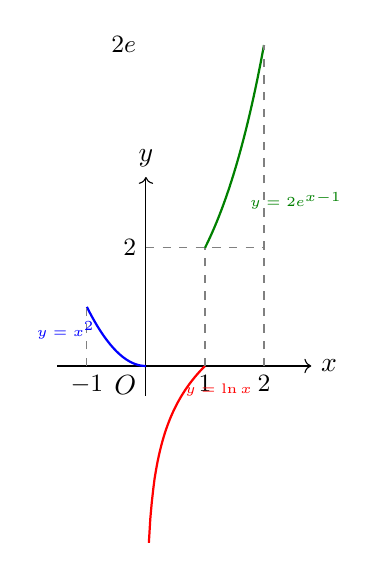
\begin{tikzpicture}[scale=0.75]
      \draw[->] (-1.5,0) -- (2.8,0) node[right] {$x$};
      \draw[->] (0,-0.5) -- (0,3.2) node[above] {$y$};
      % Branch 1: y = x^2 on [-1, 0)
      \draw[thick,blue,domain=-1:0,samples=40] plot (\x,{\x*\x});
      % Branch 2: y = ln x on (0, 1]
      \draw[thick,red,domain=0.05:1,samples=40] plot (\x,{ln(\x)});
      % Branch 3: y = 2*exp(x-1) on (1, 2]
      \draw[thick,green!50!black,domain=1:2,samples=30] plot (\x,{2*exp(\x-1)});
      % Key points and dashed lines
      \draw[dashed,gray] (-1,0)--(-1,1);
      \draw[dashed,gray] (1,0)--(1,2);
      \draw[dashed,gray] (2,0)--(2,{2*exp(1)});
      \draw[dashed,gray] (0,2)--(2,2);
      \node[below] at (-1,0) {\small $-1$};
      \node[below] at (1,0) {\small $1$};
      \node[below] at (2,0) {\small $2$};
      \node[left] at (0,2) {\small $2$};
      \node[left] at (0,{2*exp(1)}) {\small $2e$};
      \node[below left] at (0,0) {$O$};
      % Labels
      \node[blue,left] at (-0.7,0.6) {\tiny $y=x^2$};
      \node[red,right] at (0.5,-0.4) {\tiny $y=\ln x$};
      \node[green!50!black,right] at (1.6,2.8) {\tiny $y=2e^{x-1}$};
    \end{tikzpicture}
  \end{center}
\end{frame}

% ============================================================
\subsection{Summary \& Challenge Problems}
% ============================================================

% -------------------- Summary --------------------
\begin{frame}{Section Summary}
  \begin{enumerate}
    \item<1-> \textbf{Definition of a function:} three elements --- domain, correspondence rule, range.
    \item<2-> \textbf{Key properties:} boundedness, monotonicity, even/odd parity, periodicity.
    \item<3-> \textbf{Structure of elementary functions:} built from five basic classes via finite operations and composition.
    \item<4-> \textbf{Inverse \& composite functions:} existence conditions, properties, techniques for piecewise cases.
  \end{enumerate}
\end{frame}

% -------------------- Backup Problem 1 --------------------
\begin{frame}{Challenge Problem 1: Proving Oddness}
  \begin{example}
    Suppose $f(0)=0$ and for $x\neq 0$:
    \[
      a\,f(x)+b\,f\!\left(\frac{1}{x}\right)=\frac{c}{x},
    \]
    where $a,b,c$ are constants with $|a|\neq|b|$.
    Prove that $f(x)$ is an odd function.
  \end{example}
  \pause
  \begin{block}{Step 1: Set Up the System}
    Substitute $t=\dfrac{1}{x}$ to obtain a second equation:
    \[
      \begin{cases}
        a\,f(x)+b\,f(1/x)=c/x,\\[4pt]
        a\,f(1/x)+b\,f(x)=cx.
      \end{cases}
    \]
  \end{block}
\end{frame}

\begin{frame}{Challenge Problem 1: Solution (cont.)}
  \begin{block}{Step 2: Eliminate $f(1/x)$}
    Solving the linear system for $f(x)$:
    \[
      f(x)=\frac{c}{b^2-a^2}\!\left(bx-\frac{a}{x}\right)\;(x\neq0).
    \]
  \end{block}
  \pause
  \begin{alertblock}{Conclusion}
    Clearly $f(-x)=-f(x)$ and $f(0)=0$.\\
    Therefore $f(x)$ is an \textbf{odd function}. \hfill$\blacksquare$
  \end{alertblock}
\end{frame}

% -------------------- Backup Problem 2 --------------------
\begin{frame}{Challenge Problem 2: Symmetry Implies Periodicity}
  \begin{example}
    Let $y=f(x)$, $x\in(-\infty,+\infty)$.
    If the graph is symmetric about both $x=a$ and $x=b$ ($a\neq b$),
    prove that $f(x)$ is periodic.
  \end{example}
  \pause
  \begin{block}{Step 1: Symmetry Conditions}
    \[
      f(a+x)=f(a-x),\qquad f(b+x)=f(b-x).
    \]
  \end{block}
  \pause
  \begin{block}{Step 2: Apply Symmetry Twice}
    \begin{align*}
      f(x)&=f[a+(x-a)]=f[a-(x-a)]=f(2a-x)\\
          &=f[b+(2a-x-b)].
    \end{align*}
  \end{block}
\end{frame}

\begin{frame}{Challenge Problem 2: Proof (cont.)}
  Continuing from the previous step:
  \pause
  \begin{block}{Step 3: Second Reflection}
    \[
      f[b-(2a-x-b)] = f[x+2(b-a)].
    \]
  \end{block}
  \pause
  \begin{alertblock}{Conclusion}
    Hence $f(x)$ is periodic with \textbf{period $T=2(b-a)$}. \hfill$\blacksquare$
  \end{alertblock}
  \vfill
  \small
  \textit{Key idea:} Two reflections about distinct vertical axes compose to a horizontal translation.
\end{frame}

% ==================== END ====================
\begin{frame}
  \centering
  \vfill
  {\Large\bfseries End of Section 1}\\[8pt]
  {\normalsize Mappings and Functions}
  \vfill
\end{frame}

\end{document}
